\section{Data Science Concepts}

\subsection{Linear Regression Visualization}

\begin{figure}[H]
\centering
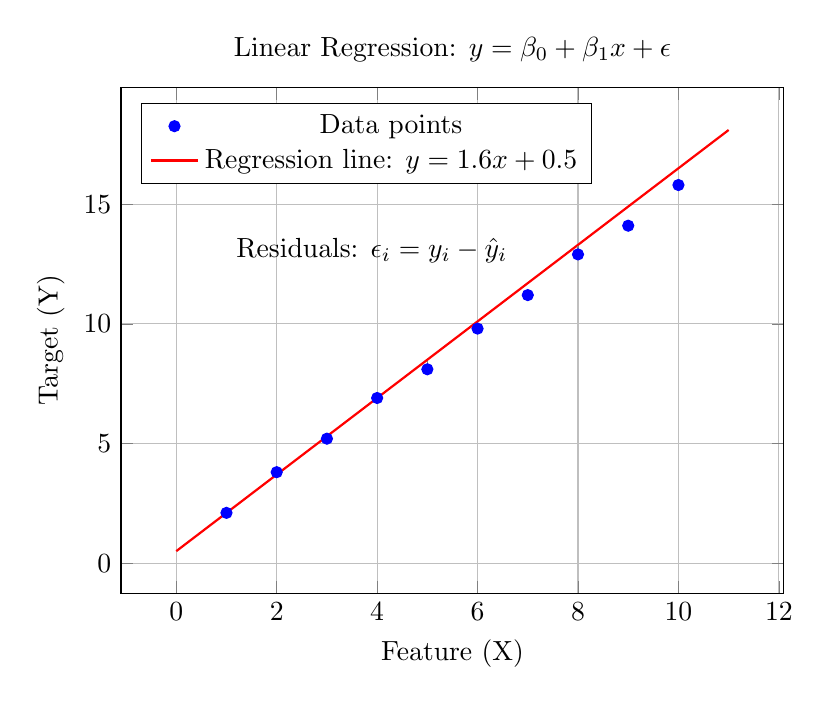
\begin{tikzpicture}
\begin{axis}[
    width=10cm,
    height=8cm,
    xlabel={Feature (X)},
    ylabel={Target (Y)},
    title={Linear Regression: $y = \beta_0 + \beta_1x + \epsilon$},
    grid=major,
    legend pos=north west,
    scatter/classes={a={blue}},
    axis equal=false
]

% Generate some sample data points with noise
\addplot[scatter, only marks, scatter src=explicit symbolic, 
         mark=*, blue, mark size=2] 
table {
x y
1 2.1
2 3.8
3 5.2
4 6.9
5 8.1
6 9.8
7 11.2
8 12.9
9 14.1
10 15.8
};

% Add linear regression line (y = 1.6x + 0.5)
\addplot[red, thick, domain=0:11, samples=2] {1.6*x + 0.5};
\addlegendentry{Data points}
\addlegendentry{Regression line: $y = 1.6x + 0.5$}

% Add some error bars/residuals
\draw[dashed, gray] (axis cs:2,3.8) -- (axis cs:2,3.7);
\draw[dashed, gray] (axis cs:5,8.1) -- (axis cs:5,8.5);
\draw[dashed, gray] (axis cs:8,12.9) -- (axis cs:8,13.3);

% Add equation annotation
\node[anchor=south west] at (axis cs:1,16) {$\hat{y} = \beta_0 + \beta_1x$};
\node[anchor=north west] at (axis cs:1,14) {Residuals: $\epsilon_i = y_i - \hat{y}_i$};

\end{axis}
\end{tikzpicture}
\caption{Linear Regression: Fundamental data science concept showing the relationship between a feature (X) and target variable (Y) with best-fit line and residuals.}
\label{fig:linear-regression}
\end{figure}
